\section{\hard\ 谱序列}

\epigraph
  {这场\trCohomology{}的洪水令我有点惊慌失措，但我勇敢地挺住了。你的%
   \trSpectralSequence{}在我看来是合理的（我原以为在一个特殊情形里证明了它不成立，
   但我弄错了——恰恰相反，它运转得漂亮极了）。}
  {——J.-P.~\trSerre，致 A.~\trGrothendieck{}的信，1956 年 3 月 14 日，[GrS, p.~38]}

\trSpectralSequence{}是一件强有力的记账工具，用于证明涉及复杂\trCommutativeDiagram{}的命题。它们由\trLeray{}于 20 世纪 40 年代引入，与\trSheaf{}的引入同时。它们素有晦涩艰难之名。有人提出：「谱」这个名号之所以得来，是因为\trSpectralSequence{}如同鬼魅，可畏、邪恶而危险。%
\footnote{译注：英文 spectral（谱）与 specter（鬼魅）同词根，作者借谐音打趣。}
我从未听见有人反对这一解读；这或许并不奇怪，因为这一解读正是我方才杜撰的。

尽管如此，本节的目标是向你讲够多的东西，使你能毫无犹疑、毫无畏惧地使用\trSpectralSequence，并使你明白：当它们在讨论班上露面时，你为何不必害怕。这套讲法也许与众不同之处在于：我们将用\trSpectralSequence{}去证明一些你或许早已见过、而且用别的方式也能轻松证明的事情；这能让你在如何使用它们上获得一些上手经验。我们也只在\trDoubleComplex{}这一特殊情形中与它们打交道（这是代数几何中迄今最常用到的版本），而不涉及通常陈述的一般形式（\trFiltered{}复形、正合偶等）。想了解更多细节，可参看 [Weib, Ch.~5]。

阅读本章其余部分时，你不要读本节；恰当的做法是，在你第一次需要用到它之前再读它。而当你终于来读这一节时，\cref{ex:ses-cohomology-les}及其之前的练习你必须全做。

为具体起见，我们在环 $A$ 上\trModule{}的范畴 $\catMod{A}$ 中工作。不过，我们所说的一切在任何\trAbelianCategory{}中都成立。（如果这能让你更安心，你也可以改在域 $k$ 上\trVectorSpace{}的范畴 $\catVec{k}$ 中工作。）

\textbf{1.6.1. \trDoubleComplex。}\quad 一个\textbf{\trDoubleComplex}（double complex）是一族 $A$-\trModule{} $E^{p,q}$（$p,q\in\mathbb{Z}$），连同「向右」的态射 $d^{p,q}_{\to}\colon E^{p,q}\to E^{p+1,q}$ 与「向上」的态射 $d^{p,q}_{\uparrow}\colon E^{p,q}\to E^{p,q+1}$。在上标中，第一个指标表示列数（「$x$ 坐标」），第二个指标表示行数（「$y$ 坐标」）。（警示：这与矩阵的习惯相反。）下标意在提示箭头的方向。我们将永远把它们写作 $d_{\to}$ 与 $d_{\uparrow}$，并省去上标。我们要求 $d_{\to}$ 与 $d_{\uparrow}$ 满足：(a)~$d_{\to}^{2}=0$；(b)~$d_{\uparrow}^{2}=0$；外加一条：(c)~要么 $d_{\to}d_{\uparrow}=d_{\uparrow}d_{\to}$（所有方格都交换），要么 $d_{\to}d_{\uparrow}+d_{\uparrow}d_{\to}=0$（它们全都\trAnticommute）。两种情形都在自然界出现；从一种换到另一种，只需把 $d^{p,q}_{\uparrow}$ 换成 $(-1)^{p}d^{p,q}_{\uparrow}$。所以我将假定所有方格都\trAnticommute，并假定你知道如何把交换的情形化归为这种情形。（你会看到，就这套做法而言并无区别；缘由基本上是：同态 $f$ 的像与核分别等于 $-f$ 的像与核。）
\[
\begin{tikzcd}[row sep=2.0em, column sep=3.2em]
E^{p,q+1} \ar[rr,"d_{\to}^{\,p,q+1}"] \ar[dd,"d_{\uparrow}^{\,p,q}"'] & \text{\trAnticommute} & E^{p+1,q+1} \ar[dd,"d_{\uparrow}^{\,p+1,q}"] \\
 & & \\
E^{p,q} \ar[rr,"d_{\to}^{\,p,q}"'] & & E^{p+1,q}
\end{tikzcd}
\]

这个定义有种种变体，比如：竖直箭头向下的情形；又如要求 $E^{p,q}$ 的某个子集为零的情形。

由这个\trDoubleComplex{}我们构造相应的（单）\trComplexN{} $E^{\bullet}$：令 $E^{k}=\bigoplus_{i}E^{i,k-i}$，并取 $d=d_{\to}+d_{\uparrow}$。换言之，当只有一个上标 $k$ 时，我们指的是\trDoubleComplex{}第 $k$ 条\trAntidiagonal{}上各项之和。这个单复形有时称为\textbf{\trTotalComplex}（total complex）。注意 $d^{2}=(d_{\to}+d_{\uparrow})^{2}=d_{\to}^{2}+(d_{\to}d_{\uparrow}+d_{\uparrow}d_{\to})+d_{\uparrow}^{2}=0$，故 $E^{\bullet}$ 的确是一个\trComplexN。

单复形的\trCohomology{}有时称为该\trDoubleComplex{}的\textbf{\trHypercohomology}（hypercohomology）。我们则改用「\trDoubleComplex{}的\trCohomology」这一说法。

我们最初的目标将是求出\trDoubleComplex{}的\trCohomology。你稍后会看到，我们其实还暗藏着别的目标。

\trSpectralSequence{}是这样一张「配方」：借它可算出\trDoubleComplex{}的\trCohomology{}的某些信息。完整的配方我暂不给出。出人意料的是，这一星半点的信息已足以证明许多事情。

\textbf{1.6.2. 近似定义。}\quad 一个带右行\trOrientation{}的\trSpectralSequence{}是一列表或\trPage{}（$p,q\in\mathbb{Z}$）：$\Eto{p,q}{0}$, $\Eto{p,q}{1}$, $\Eto{p,q}{2}$, $\dots$，其中 $\Eto{p,q}{0}=E^{p,q}$，连同微分
\[
{}_{\to}d^{p,q}_{r}\colon {}_{\to}E^{p,q}_{r}\longrightarrow{}_{\to}E^{p-r+1,q+r}_{r}
\]
（$r\in\mathbb{Z}_{\ge0}$），满足 ${}_{\to}d^{p,q}_{r}\circ{}_{\to}d^{p+r-1,q-r}_{r}=0$，并且 ${}_{\to}d_{r}$ 在 $\Eto{p,q}{r}$ 处取的\trCohomology（即 $\ker{}_{\to}d^{p,q}_{r}\big/\im{}_{\to}d^{p+r-1,q-r}_{r}$）与 $\Eto{p,q}{r+1}$ 之间有一个同构。

这条\trOrientation{}表明：我们的第 $0$ 个微分正是向右的那个：$d_{0}=d_{\to}$。左下标「$\to$」通常省去不写。

这些态射的先后次序，最好直观地看：
\begin{equation*}\tag{1.6.2.1}\label{eq:ss-right-arrows}
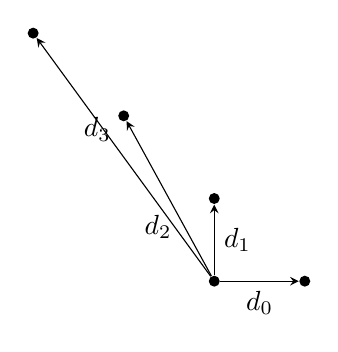
\begin{tikzpicture}[>=stealth,dot/.style={circle,fill,inner sep=1.4pt}]
  \node[dot] (o)  at (0,0)       {};
  \node[dot] (t0) at (1.15,0)    {};
  \node[dot] (t1) at (0,1.05)    {};
  \node[dot] (t2) at (-1.15,2.1) {};
  \node[dot] (t3) at (-2.3,3.15) {};
  \draw[->] (o) -- (t0) node[midway,below] {$d_0$};
  \draw[->] (o) -- (t1) node[midway,right] {$d_1$};
  \draw[->] (o) -- (t2) node[pos=0.42,below left=-2pt] {$d_2$};
  \draw[->] (o) -- (t3) node[pos=0.55,above left=-2pt] {$d_3$};
\end{tikzpicture}
\end{equation*}
（诸态射各自作用于不同的\trPage。）注意，按单复形 $E^{\bullet}$ 的分次来数，该映射永远是「$1$ 次」的。（这句非正式的话究竟何所指，你应当自己弄清楚。）

真正的定义描述的是 $\Eto{\bullet,\bullet}{r}$ 与 $d_{r}$ 究竟为何物——用 $\Eto{\bullet,\bullet}{0}$ 表出。下面我们将描述 $d_{0}$、$d_{1}$ 与 $d_{2}$；至于这列微分此后以某种自然方式继续，你暂且信之。

注意：对一切 $i<r$，$\Eto{p,q}{r}$ 总是第 $i$ \trPage{}上相应项 $\Eto{p,q}{i}$ 的\textbf{\trSubquotient}（subquotient）。特别地，若 $E^{p,q}=0$，则对一切 $r$ 都有 $\Eto{p,q}{r}=0$。

现在设 $E^{\bullet,\bullet}$ 是一个\textbf{\trFirstQuadrant\trDoubleComplex}（first quadrant double complex），即当 $p<0$ 或 $q<0$ 时 $E^{p,q}=0$（于是除非 $p,q\in\mathbb{Z}_{\ge0}$，对一切 $r$ 都有 $\Eto{p,q}{r}=0$）。那么对任意固定的 $p,q$，一旦 $r$ 充分大，$\Eto{p,q}{r+1}$ 便可由 $(E_{r},d_{r})$ 用复形
\begin{equation*}\tag{1.6.2.2}\label{eq:ss-stable-term-complex}
\begin{tikzcd}[row sep=3.4em, column sep=2.0em]
0 \\
   & E^{p,q}_{r} \ar[ul,"d^{p,q}_{r}"'] \\
   &    & 0, \ar[ul,"d^{p+r-1,q-r}_{r}"']
\end{tikzcd}
\end{equation*}
算出，从而我们有典范同构
\[
E^{p,q}_{r}\cong E^{p,q}_{r+1}\cong E^{p,q}_{r+2}\cong\cdots.
\]
我们将把这个\trModule{}记作 $E^{p,q}_{\infty}$。同样的想法也适用于别的情形，比如\trDoubleComplex{}只在有限多行上非零的情形——此时除非 $q_{0}<q<q_{1}$，否则 $E^{p,q}=0$。这将在例如\trMappingCone{}与\trLongExactSequence{}的讨论中出现（见下面的\cref{ex:ses-cohomology-les}与\cref{ex:mapping-cone-long-exact}）。

我们现在来显式描述\trSpectralSequence{}的头几\trPage。如上所述，$\Eto{\bullet,\bullet}{0}=E^{\bullet,\bullet}$ 上的微分 $d_{0}$ 定义为 $d_{\to}$。各行都是复形。
\[
\begin{tikzcd}[row sep=1.5em, column sep=3.0em]
 & \bullet \ar[r] & \bullet \ar[r] & \bullet \\
\text{第 0 \trPage{} $E_{0}$：} & \bullet \ar[r] & \bullet \ar[r] & \bullet \\
 & \bullet \ar[r] & \bullet \ar[r] & \bullet
\end{tikzcd}
\]
于是 $E_{1}$ 不过是「诸行的\trCohomology」构成的表。你应当验证：各行上同调群之间现在有了竖直映射 $d^{p,q}_{1}\colon E^{p,q}_{1}\to E^{p,q+1}_{1}$，由 $d_{\uparrow}$ 诱导，并且这些映射使各列成为复形。（这本质上就是「复形的映射诱导\trHomology{}上的映射」这一事实。）我们已经「用尽了水平态射」，但「竖直的微分还活着」。
\[
\begin{tikzcd}[row sep=1.9em, column sep=3.0em]
 & \bullet & \bullet & \bullet \\
\text{第 1 \trPage{} $E_{1}$：} & \bullet \ar[u] & \bullet \ar[u] & \bullet \ar[u] \\
 & \bullet \ar[u] & \bullet \ar[u] & \bullet \ar[u]
\end{tikzcd}
\]
我们取 $d_{1}$ 在 $E_{1}$ 上的\trCohomology，得到新的表 $E^{p,q}_{2}$。事实证明：从每个表项到「上方两行、左方一列」的那个表项有自然态射，而且这两个态射的复合为 $0$。（弄清这个自然态射 $d_{2}$ 应当怎样定义，是一道非常值得做的练习。你的论证也许会令你想起蛇形引理（例~1.6.5）中的\trConnectingHomomorphism，或者由\trComplexes{}的\trShortExactSequence{}产生的\trCohomology{}\trLongExactSequence{}（定理~1.5.8）中的连接同态。这绝非巧合。）
\[
\begin{tikzcd}[row sep=1.9em, column sep=3.0em]
 & \bullet & \bullet & \bullet \\
\text{第 2 \trPage{} $E_{2}$：} & \bullet & \bullet & \bullet \\
 & \bullet & \bullet \ar[uul] & \bullet \ar[uul]
\end{tikzcd}
\]
这只是一个模式的开始。

于是，这是一个定理：$\mathrm{H}^{k}(E^{\bullet})$ 有一个由 $E^{p,q}_{\infty}$（$p+q=k$）给出的\trFiltered{}。（我们尚不能把它作为正式的\trhTheorem{}来陈述，因为\trSpectralSequence{}的诸\trPage{}与诸微分还没有精确定义。）更精确地说，存在一个\trFiltered{}
\begin{equation*}\tag{1.6.2.3}\label{eq:ss-filtration}
\begin{tikzcd}[column sep=1.9em]
E^{0,k}_{\infty} \ar[r,hook,"E^{1,k-1}_{\infty}"] & ? \ar[r,hook,"E^{2,k-2}_{\infty}"] & \cdots \ar[r,hook,"E^{k,0}_{\infty}"] & \mathrm{H}^{k}(E^{\bullet})
\end{tikzcd}
\end{equation*}
其中商标在每个包含映射的上方。（有一个诀窍，可以帮你记住商应当放在哪一头。越靠后的\trPage{}上的微分，刺入\trFiltered{}越深。于是，较晚箭头所指方向上的那些项是\trSubobject，而较晚「箭尾」方向上的那些项是商。这个诀窍的好处在于不依赖\trSpectralSequence{}的细节，比如「象限」或\trOrientation。）

我们说\trSpectralSequence{} $\Eto{\bullet,\bullet}{}$ \textbf{\trConverge}（converge）到 $\mathrm{H}^{\bullet}(E^{\bullet})$；也常说 $\Eto{\bullet,\bullet}{2}$（或任何别的\trPage）\textbf{\trAbut}（abut）到 $\mathrm{H}^{\bullet}(E^{\bullet})$。

尽管\trFiltered{}只给出 $\mathrm{H}^{\bullet}(E^{\bullet})$ 的部分信息，有时却能把它精确求出。一个例子是：所有 $E^{i,k-i}_{\infty}$ 都是零，或者除一个之外全为零（比如：若 $E^{\bullet,\bullet}_{r}$ 恰有一条非零的行或列，此时人们说\trSpectralSequence{}在第 $r$ 步\textbf{\trCollapse}（collapse）；不过我们不会使用这个术语）。另一个例子是在域上\trVectorSpace{}的范畴中，此时我们能求出 $\mathrm{H}^{k}(E^{\bullet})$ 的维数。此外，走运的话，$E_{2}$（或某个更早的\trPage）已经就等于 $E_{\infty}$。

\begin{exercise}[来自第二\trPage{}的信息]\label{ex:ss-low-degree-info}
证明 $\mathrm{H}^{0}(E^{\bullet})=E^{0,0}_{\infty}=E^{0,0}_{2}$，并且
\[
0\longrightarrow E^{0,1}_{2}\longrightarrow\mathrm{H}^{1}(E^{\bullet})
\longrightarrow E^{1,0}_{2}\mathrel{\xrightarrow{\ d^{1,0}_{2}\ }}E^{0,2}_{2}
\longrightarrow\mathrm{H}^{2}(E^{\bullet})
\]
正合。
\end{exercise}


\textbf{1.6.3. 另一个\trOrientation。}\quad 你也许已经注意到：我们本可以把一切都按相反方向来做，即把水平态射与竖直态射的角色对调。此时给出\trSpectralSequence{}的那串箭头会长成这样（对比\eqref{eq:ss-right-arrows}）：
\begin{equation*}\tag{1.6.3.1}\label{eq:ss-up-arrows}
\begin{tikzpicture}[>=stealth,dot/.style={circle,fill,inner sep=1.4pt}]
  \node[dot] (o)  at (0,0)        {};
  \node[dot] (u0) at (0,1.05)     {};
  \node[dot] (r0) at (1.15,0)     {};
  \node[dot] (r1) at (2.3,-1.05)  {};
  \node[dot] (r2) at (3.45,-2.1)  {};
  \draw[->] (o) -- (u0);
  \draw[->] (o) -- (r0);
  \draw[->] (o) -- (r1);
  \draw[->] (o) -- (r2);
\end{tikzpicture}
\end{equation*}
这个\trSpectralSequence{}记作 $\Eup{\bullet,\bullet}{}$（「带上行\trOrientation」）。于是我们同样会得到 $\mathrm{H}^{\bullet}(E^{\bullet})$ 之\trFiltered{}的若干块（此时要当心 $\Eup{p,q}{\infty}$ 对应于诸子商的先后次序——它与\eqref{eq:ss-filtration}中 $\Eto{p,q}{\infty}$ 的次序相反）。警示：一般而言，$\Eto{p,q}{\infty}$ 与 $\Eup{p,q}{\infty}$ 之间并不同构。

事实上，「既可以从水平映射出发，也可以从竖直映射出发」这一观察，正是我们一路暗藏的目标。两种算法计算的是关于同一件事（$\mathrm{H}^{\bullet}(E^{\bullet})$）的信息；通常我们并不在乎最终答案——我们在乎的往往是按其中一种方式得到的那个答案，而要抵达它，恰恰要按另一种方式去做\trSpectralSequence。

\textbf{1.6.4. 例子。}\quad 我们现在可以来看这东西如何有用了。这些例子的寓意如下。过去，你证明各种涉及各种图的命题时，靠的也许是追元素。现在，你只需把它们代入一张\trSpectralSequence，让\trSpectralSequence{}机器替你追。

\textbf{1.6.5. 例：证明蛇形引理。}\quad 考虑图
\begin{equation*}\tag{1.6.5.1}\label{eq:snake-lemma-grid}
\begin{tikzcd}[row sep=2.8em, column sep=2.4em]
0 \ar[r] & D \ar[r] & E \ar[r] & F \ar[r] & 0 \\
0 \ar[r] & A \ar[u,"\alpha"] \ar[r] & B \ar[u,"\beta"] \ar[r] & C \ar[u,"\gamma"] \ar[r] & 0
\end{tikzcd}
\end{equation*}
其中两行在中间处（即在 $A,B,C,D,E,F$ 处）正合，且诸方格交换。（蛇形引理通常表述成竖直箭头朝下的样子，但我想让它迁就我的\trSpectralSequence{}约定。）

我们希望证明有正合列
\begin{equation*}\tag{1.6.5.2}\label{eq:snake-lemma-les}
0\longrightarrow\ker\alpha\longrightarrow\ker\beta\longrightarrow\ker\gamma
\longrightarrow\coker\alpha\longrightarrow\coker\beta\longrightarrow\coker\gamma\longrightarrow 0.
\end{equation*}

我们把它插进\trSpectralSequence{}机器。先用右行\trOrientation{}计算\trCohomology，即按\eqref{eq:ss-right-arrows}的次序。由于两行正合，$\Eto{p,q}{1}=0$，于是\trSpectralSequence{}已经收敛：$\Eto{p,q}{\infty}=0$。

接下来我们用另一种办法计算这个「$0$」：用上行\trOrientation{}计算\trSpectralSequence。此时 $\Eup{\bullet,\bullet}{1}$（连同其微分）为：
\[
\begin{gathered}
0\longrightarrow\coker\alpha\longrightarrow\coker\beta\longrightarrow\coker\gamma\longrightarrow 0\\[14pt]
0\longrightarrow\ker\alpha\longrightarrow\ker\beta\longrightarrow\ker\gamma\longrightarrow 0.
\end{gathered}
\]
于是 $\Eup{\bullet,\bullet}{2}$ 形如：
\[
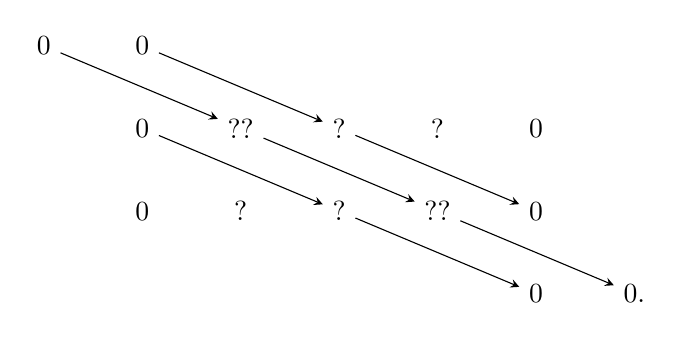
\begin{tikzpicture}[>=stealth,x=1.25cm,y=1.05cm]
  \node (a0) at (0,2)  {$0$};
  \node (a1) at (1,2)  {$0$};
  \node (b0) at (1,1)  {$0$};
  \node (b1) at (2,1)  {$??$};
  \node (b2) at (3,1)  {$?$};
  \node (b3) at (4,1)  {$?$};
  \node (b4) at (5,1)  {$0$};
  \node (c0) at (1,0)  {$0$};
  \node (c1) at (2,0)  {$?$};
  \node (c2) at (3,0)  {$?$};
  \node (c3) at (4,0)  {$??$};
  \node (c4) at (5,0)  {$0$};
  \node (e0) at (5,-1) {$0$};
  \node (e1) at (6,-1) {$0.$};
  \draw[->] (a0) -- (b1);
  \draw[->] (a1) -- (b2);
  \draw[->] (b0) -- (c2);
  \draw[->] (b1) -- (c3);
  \draw[->] (b2) -- (c4);
  \draw[->] (c2) -- (e0);
  \draw[->] (c3) -- (e1);
\end{tikzpicture}
\]
我们看到：$\Eup{}{2}$ 之后，除双问号外的一切项都将稳定下来——通向与来自单问号的映射，都是通向与来自 $0$ 项的。而 $\Eup{}{3}$ 之后，连那两个双问号项也将稳定。但最终我们的复形必是零复形。这意味着：在 $\Eup{}{2}$ 中，除那两个双问号外，一切项必为零，而且这两个双问号必彼此同构。这意味着：$0\to\ker\alpha\to\ker\beta\to\ker\gamma$ 与 $\coker\alpha\to\coker\beta\to\coker\gamma\to 0$ 都正合（这来自单问号的消失），而且
\[
\coker(\ker\beta\to\ker\gamma)\cong\ker(\coker\alpha\to\coker\beta)
\]
是同构（这来自双问号的相等）。合在一起，我们便证明了\eqref{eq:snake-lemma-les}的正合性，从而证明了蛇形引理！（注意：到头来，我们并不真的在乎那个\trDoubleComplex；我们只是把它当作证明蛇形引理的一件道具。）

\trSpectralSequence{}使人容易看清如何把结果进一步推广。例如，若不再假设 $A\to B$ 是\trInjectiveMap，结论将如何改变？

\begin{exercise}[不重要的练习：嫁接正合列，蛇形引理的一个变体]\label{ex:grafting-snake-variant}
把蛇形引理作如下扩充。设有交换图
\[
\begin{tikzcd}[row sep=2.8em, column sep=2.4em]
 & 0 \ar[r] & X' \ar[r] & Y' \ar[r] & Z' \ar[r] & A' \ar[r] & \cdots \\
\cdots \ar[r] & W \ar[u] \ar[r] & X \ar[u,"a"] \ar[r] & Y \ar[u,"b"] \ar[r] & Z \ar[u,"c"] \ar[r] & 0 \ar[u] &
\end{tikzcd}
\]
其中上行与下行都正合。证明：上行与下行可以「嫁接」在一起，得到正合列
\[
\begin{array}{l}
\cdots\longrightarrow W\longrightarrow\ker a\longrightarrow\ker b\longrightarrow\ker c\\[10pt]
\hspace*{5.5em}\longrightarrow\coker a\longrightarrow\coker b\longrightarrow\coker c\longrightarrow A'\longrightarrow\cdots.
\end{array}
\]
\end{exercise}

\textbf{1.6.6. 例：五引理。}\quad 设
\begin{equation*}\tag{1.6.6.1}\label{eq:five-lemma-grid}
\begin{tikzcd}[row sep=2.8em, column sep=2.2em]
F \ar[r] & G \ar[r] & H \ar[r] & I \ar[r] & J \\
A \ar[u,"\alpha"] \ar[r] & B \ar[u,"\beta"] \ar[r] & C \ar[u,"\gamma"] \ar[r] & D \ar[u,"\delta"] \ar[r] & E \ar[u,"\epsilon"]
\end{tikzcd}
\end{equation*}
其中两行正合，且诸方格交换。

设 $\alpha$、$\beta$、$\delta$、$\epsilon$ 都是\trIsomorphism。我们将证明 $\gamma$ 是\trIsomorphism。

先用右行\trOrientation{}\eqref{eq:ss-right-arrows}计算全复形的\trCohomology。这样选，是因为我们看得出会得到一大堆零。此时 $\Eto{\bullet,\bullet}{1}$ 长这样：
\[
\begin{tikzcd}[row sep=2.4em, column sep=2.4em]
? & 0 & 0 & 0 & ? \\
? \ar[u] & 0 \ar[u] & 0 \ar[u] & 0 \ar[u] & ? \ar[u]
\end{tikzcd}
\]
于是 $\Eto{}{2}$ 看上去类似，而且序列将在 $E_{2}$ 处收敛，因为此后表中再也不会出现两个非零项之间的箭头。我们不能断言全复形的\trCohomology{}为零，但可以注意到：它在除四个次数之外的所有次数上都为零——而最重要的是，它在对应于表项 $C$ 与 $H$（$\gamma$ 的\trSource{}与\trTarget）的那两个次数上为零。

接下来用上行\trOrientation{}\eqref{eq:ss-up-arrows}来计算它。此时 $\Eup{}{1}$ 长这样：
\[
\begin{tikzcd}[row sep=3.0em, column sep=2.0em]
0 \ar[r] & 0 \ar[r] & ? \ar[r] & 0 \ar[r] & 0 \\
0 \ar[r] & 0 \ar[r] & ? \ar[r] & 0 \ar[r] & 0,
\end{tikzcd}
\]
而\trSpectralSequence{}就在这一步收敛。我们希望证明那两个问号为零。但它们恰恰是全复形的\trCohomology{}中我们刚刚证明了为零的那两个——于是证毕！

要熟悉这类论证，最好的办法是亲自把它试上几遍，并体会到它确实容易。所以下面的练习你应当去做！其中许多本可以直接做出，但你应当刻意试着使用这套\trSpectralSequence{}机器，以此练手并建立信心。

\begin{exercise}[更微妙的五引理]\label{ex:five-lemma-weakening}
观察上面五引理的\trSpectralSequence{}证明，证明它的一个更微妙的版本：可以把其中一个\trIsomorphism{}的假设减弱为只要求\trInjection，把另一个减弱为只要求\trSurjectiveMap。（我故意不说出是哪两个，好让你亲眼看到\trSpectralSequence{}如何告诉你怎样改进这个结果。）
\end{exercise}

\begin{exercise}[五引理的另一个微妙版本]\label{ex:five-lemma-partial-iso}
若\eqref{eq:five-lemma-grid}中的 $\beta$ 与 $\delta$ 都是\trInjectiveMap，而 $\alpha$ 是\trSurjectiveMap，证明 $\gamma$ 是\trInjectiveMap。请陈述对偶的命题（其证明当然本质上相同）。
\end{exercise}

下面两个练习不再涉及\trFirstQuadrant\trDoubleComplex。你须略加思考，方能明白为何没有理由为此困惑或惊慌。

\begin{exercise}[重要练习：\trMappingCone]\label{ex:mapping-cone-long-exact}
设 $\mu\colon A^{\bullet}\to B^{\bullet}$ 是\trComplexes{}的一个态射。设 $C^{\bullet}$ 是与\trDoubleComplex{} $A^{\bullet}\to B^{\bullet}$ 相伴的单复形。（$C^{\bullet}$ 称为 $\mu$ 的\textbf{\trMappingCone}（mapping cone）。）证明存在\trComplexes{}的\trLongExactSequence：
\[
\cdots\longrightarrow\mathrm{H}^{i-1}(C^{\bullet})\longrightarrow\mathrm{H}^{i}(A^{\bullet})\longrightarrow\mathrm{H}^{i}(B^{\bullet})\longrightarrow\mathrm{H}^{i}(C^{\bullet})\longrightarrow\mathrm{H}^{i+1}(A^{\bullet})\longrightarrow\cdots.
\]
（这里有一点记号上的含混：依你对\trDoubleComplex{}的指标约定，你的\trLongExactSequence{}看上去可能略有不同。）特别地，我们将用到如下事实：$\mu$ 在\trCohomology{}上诱导\trIsomorphism，当且仅当\trMappingCone{}正合。（我们要到定理~18.2.4 的证明中才会用到它。）
\end{exercise}

\begin{exercise}\label{ex:ses-cohomology-les}
用\trSpectralSequence{}证明：\trComplexes{}的\trShortExactSequence{}给出\trCohomology{}的\trLongExactSequence{}（定理~1.5.8）。（这是\cref{ex:mapping-cone-long-exact}的推广。）
\end{exercise}

\trGrothendieck{}的函子复合\trSpectralSequence{}（定理~23.3.5）将是\trSpectralSequence{}的一个重要例子，它能在许多有用的方向上特殊化。

至此，你可以走向世界，随心所欲地使用\trSpectralSequence{}了！

\textbf{1.6.7. \trSpectralSequence{}的完整定义与证明。}\quad 在读完上面的\trSpectralSequence{}引介之后，你可千万别在近期就去读\trSpectralSequence{}的精确定义，以及「它们果然如宣称的那样工作」的证明。但隔上一段合适的时间之后，你至少应当把某个构造与证明翻阅一遍，好让自己相信：其中并没有什么花哨的东西。这个想法并不像你以为的那样糟；见 [Vak2]。

值得注意的是，证明蕴涵\trSpectralSequence{}在第 $0$ \trPage{}上是函子性的：\trSpectralSequence{}的形式体系在\trDoubleComplex{}上具有良好的函子性质。遗憾的是，\trGrothendieck{}的术语「\trSpectralFunctor」（spectral functor）[Gr1, \S2.4] 未能流行开来。

